\documentclass[a4paper, 12pt]{article}
%\usepackage{mathtext}
\usepackage{cmap}
\usepackage[english, russian]{babel}
\usepackage[T2A]{fontenc}
\usepackage[utf8]{inputenc}
\usepackage[left=2cm, right=1.5cm, top=2cm, bottom=2cm]{geometry}
\usepackage{amsmath}
\usepackage{etoolbox}
\usepackage{amsthm}
\usepackage{amsfonts}
%\usepackage{indentfirst}
\usepackage{soul}
\usepackage{graphicx}
\usepackage{enumerate}
\usepackage{nicematrix}
\usepackage{booktabs}
\usepackage{mathtools,amssymb}

\usepackage{tikz,amstext}
\newlength{\tempheight}
\newcommand{\Let}[0]{%
	\mathbin{\text{\settoheight{\tempheight}{\mathstrut}\raisebox{0.5\pgflinewidth}{%
				\tikz[baseline,line cap=round,line join=round] \draw (0,0) --++ (0.4em,0) --++ (0,1.5ex) --++ (-0.4em,0);%
}}}}

\renewcommand{\phi}{\varphi}
\renewcommand{\epsilon}{\varepsilon}
\newcommand*\circled[1]{\tikz[baseline=(char.base)]{
            \node[shape=circle,draw,inner sep=2pt] (char) {#1};}}
\newcommand{\aug}{\fboxsep=-\fboxrule\!\!\!\fbox{\strut}\!\!\!}
\newcommand\tab[1][.5cm]{\hspace*{#1}}
\newcommand\undermat[2]{\makebox[0pt][l]{$\smash{\underbrace
			{\phantom{\begin{matrix}#2\end{matrix}}}_{\text{$#1$}}}$}#2}
\newcommand\overmat[2]{\makebox[0pt][l]{$\smash{\overbrace
			{\phantom{\begin{matrix}#2\end{matrix}}}^{\text{$#1$}}}$}#2}

\newcounter{lemcount}
\newcounter{lemcount2}
\newcounter{thcount}
\theoremstyle{definition}
\newtheorem*{definition}{Определение}
\newtheorem*{theorem}{Теорема}
\newtheorem*{consequense}{Следствие}
\newtheorem*{lemma}{Лемма}
\newtheorem*{subtheorem}{Утверждение}
\newtheorem*{formula}{Вывод формулы}
\newtheorem*{formulas}{Вывод формул}
\newtheorem*{remark}{Замечание}
\newtheorem*{examples}{Примеры}
\newtheorem*{example}{Пример}
\newtheorem*{lalala}{Упражнение}
\newtheorem*{algorithm}{Алгоритм}
\newtheorem*{properties}{Свойства}
\newtheorem*{properties1}{Свойство}
\newtheorem{lemmanum}[lemcount]{Лемма}
\newtheorem{lemmanum2}[lemcount2]{Лемма}
\newtheorem{theoremnum}[thcount]{Теорема}
% \newtheorem{theoremL}{Теорема}[section]
\usepackage[T2A]{fontenc}
\usepackage[utf8]{inputenc}
\usepackage[russian]{babel}
\addto\captionsenglish{% Replace "english" with the language you use
	\renewcommand{\contentsname}%
	{Содержание}%
}

\newsavebox{\boxedalignbox}
\newenvironment{boxedalign*}
  {\begin{equation*}\begin{lrbox}{\boxedalignbox}$\begin{aligned}}
  {\end{aligned}$\end{lrbox}\fbox{\usebox{\boxedalignbox}}\end{equation*}}

\usepackage{titlesec}
\titleformat{\section}{\LARGE \bfseries}{\thesection}{1em}{}
\titleformat{\subsection}{\Large\bfseries}{\thesubsection}{1em}{}
\titleformat{\subsubsection}{\large\bfseries}{\thesubsubsection}{1em}{}

\usepackage{hyperref}
\usepackage{xcolor}
% Цвета для гиперссылок
\definecolor{linkcolor}{HTML}{225ae2} % цвет ссылок
\definecolor{urlcolor}{HTML}{225ae2} % цвет гиперссылок
\hypersetup{
	pdfstartview=FitH, 
	linkcolor=linkcolor,
	urlcolor=urlcolor,
	colorlinks=true
}
\usetikzlibrary{calc}

\begin{document}

\section{(50 билет) Поверхности второго порядка}


\subsection{Общее уравнение}
\begin{definition}
    Поверхностью второго порядка называется множество точек трёхмерного аффинного или точечно-евклидова пространства, координаты которых в некоторой аффинной системе координат удовлетворяют уравнению $F(x, y, z) = 0$, где
    \[ F(x, y, z) = a_{11} x^2 + a_{22} y^2 + a_{33} z^2 + 2a_{12} xy + 2a_{13} xz + 2a_{23} yz + 2a_1 x + 2a_2 y + 2a_3 z + a_0 \]
    причём хотя бы одно из чисел $a_{11}, \ a_{22}, \ a_{33}, \ a_{12}, \ a_{13}, \ a_{23}$ отлично от нуля. Выражение $F(x, y, z)$ - \textit{многочлен второй степени} от переменных $x, y, z$.
    Уравнение $F(x, y, z) = 0$ называется \textit{общим уравнением} поверхности второго порядка.
\end{definition}

\begin{remark}
    Точно так же определяются повехности второго порядка в аффинном или точечно-евклидовом пространстве произвольной конечной размерности $n$;
    они задаются многочленами второй степени от $n$ переменных.
\end{remark}

Теория поверхностей второго порядка аналогична теории кривых второго порядка.


\subsection{Квадратичная часть и матрицы}
С каждым многочленом $F(x,y,z)$ связано \textit{квадратичное отображение} пространства (с данной системой координат) $f: A^3 \to \mathbb{R}$, которое каждой точке $X$ с координатами $(x, y, z)$ ставит в соответствие число $F(x,y,z)$.
Говорят, что это отображение представлено многочленом $F$ в данной системе координат.
В другой системе координат многочлен, представляющий ту же функцию, станет другим.

Как и в случае линий второго порядка:
\[ F(x,y,z) = \begin{pmatrix}
    x & y & z & 1
\end{pmatrix}
A
\begin{pmatrix}
    x \\ y \\ z \\ 1
\end{pmatrix}
=
\begin{pmatrix}
    x & y & z
\end{pmatrix}
A_1
\begin{pmatrix}
    x \\ y \\ z
\end{pmatrix} 
+ 2 \begin{pmatrix}
    x & y & z
\end{pmatrix}
\begin{pmatrix}
    a_1 \\ a_2 \\ a_3
\end{pmatrix} 
+ a_0,
\]
где
\[ A =
\begin{pmatrix}
    a_{11} & a_{12} & a_{13} & a_{1} \\
    a_{12} & a_{22} & a_{23} & a_{2} \\
    a_{13} & a_{23} & a_{33} & a_{3} \\
    a_{1} & a_{2} & a_{3} & a_{0} \\
\end{pmatrix}
\] – большая матрица,
\[ A_1 =
\begin{pmatrix}
    a_{11} & a_{12} & a_{13} \\
    a_{12} & a_{22} & a_{23} \\
    a_{13} & a_{23} & a_{33} \\
\end{pmatrix}
\] – малая матрица (квадратичной части).

\begin{definition}
    \[ F_1(x, y, z) = a_{11} x^2 + a_{22} y^2 + a_{33} z^2 + 2a_{12} xy + 2a_{13} xz + 2a_{23} yz\]
    называется \textit{квадратичной частью} многочлена $F$.
\end{definition}


\subsection{Закон изменения матриц при переходе к новой аффинной системе координат}
Дословно так же, как в случае линий, доказывается, что при переходе к новой системе координат матрицы $A$ и $A_1$ многочлена $F$, представляющие всё ту же функцию $f: A^3 \to \mathbb{R}$, меняются по закону $A_1^{'} = C^T A_1 C$ и $A^{'} = D^T A D$, где $A_1^{'}$ и $A^{'}$ – матрицы в новых координатах, $C$ – матрица перехода от старого базиса к новому (её столбцы – координаты новых базисных векторов в старом базисе),
$D = \begin{pNiceMatrix}\Block{3-3}<\Huge>{C}&&&x_0\\&&&y_0\\&&&z_0\\0&0&0&1\end{pNiceMatrix}$, где
$x_0, y_0, z_0$ - координата нового начала координат в старой системе координат.

В новой системе координат:
\[ F^{'}(x^{'},y^{'},z^{'}) = \begin{pmatrix}
    x^{'} & y^{'} & z^{'} & 1
\end{pmatrix}
A^{'}
\begin{pmatrix}
    x^{'} \\ y^{'} \\ z^{'} \\ 1
\end{pmatrix}
+ 2 \begin{pmatrix}
    x^{'} & y^{'} & z^{'}
\end{pmatrix}
A_1^{'}
\begin{pmatrix}
    a_1^{'} \\ a_2^{'} \\ a_3^{'}
\end{pmatrix} 
+ a_0,
\]
где буквы со штрихами – координаты, многочлен и матрицы в новой системе координат,

\[
\begin{pmatrix}
    a_1^{'} \\ a_2^{'} \\ a_3^{'}
\end{pmatrix} = C^T 
\begin{pmatrix}
    a_1 \\ a_2 \\ a_3
\end{pmatrix}.
\]


\section{(51 билет) Приведение уравнений поверхностей второго порядка к каноническому виду}


\subsection{Алгоритм приведения уравнения к каноническому виду}
Будем считать, что дело происходит в точечно-евклидовом пространстве $\mathbb{R}^3$ и многочлен $F$, представляющий квадратичное отображение $f: \mathbb{R}^3 \to \mathbb{R}$, задан в прямоугольной системе координат. Это не умаляет общности: если задана не прямоугольная система координат, то мы всегда можем перейти в прямоугольную (по выписанным выше формулам), а если дело происходит в аффинном пространстве, то мы можем временно превратить его в евклидово, определив скалярное произведение в данной системе координат (в которой записана функция $F(x,y,z)$) по формуле $\left(
     \begin{pmatrix}
        x_1 \\ y_1 \\ z_1
     \end{pmatrix},
     \begin{pmatrix}
        x_2 \\ y_2 \\ z_2
     \end{pmatrix}
\right)
= x_1 x_2 + y_1 y_2 + z_1 z_2$.
Эта формула действительно задаёт некоторое скалярное произведение, и наша система координат прямоугольна относительно него.

Совершенно так же (и из тех же соображений), как в случае линий, мы можем найти каноническую систему координат (прямоугольную!), в которой уравнение поверхности имеет простейший вид:

\begin{enumerate}
    \item Решаем характеристическое уравнение $|A - \lambda E| = 0$, находим корни $\lambda_1, \lambda_2, \lambda_3$ - характеристические числа (собственные значения).
    
    В этом месте отличие (от случая линии): если нулевых корней $\leqslant 1$, то первые номера даём положительным $\lambda$ (упорядочиваем по возрастанию), следующие – отрицательным (по убыванию), потом идёт 0 (если есть). Если получилось два нулевых корня, то $\lambda_1 = \lambda_3 = 0, \ \lambda_2 \neq 0$.
    \item Для каждого $i = 1, 2, 3$ решаем однородную систему уравнений $(A - \lambda_i E) \begin{pmatrix} x \\ y \\ z \end{pmatrix} = \begin{pmatrix} 0\\0\\0 \end{pmatrix}$, находим ненулевое решение (оно обязательно существует, так как $|A - \lambda_i E| = 0$). Если есть несколько линейно независимых решений (два или три), выбираем максимально возможное число линейно независимых решений так, чтобы они были взаимно ортогональны;
    другими словами, выбираем ортогональный базис в пространстве решений (мы знаем, что это возможно, поскольку какой-то базис есть всегда, а ортогонализировать базисы мы уже научились).
    \item Нормируем полученные на предыдущем шаге решения (собственные векторы, соответствующие собственным значениям $\lambda_1, \lambda_2, \lambda_3$):
    если $\bar{u_i}$ – решение, соответствующее числу $\lambda_i$, то полагаем $\bar{e_i^{'}} = \frac{\bar{u_i}}{|\bar{u_i}|}$.
    Векторы $\bar{e_1^{'}}, \bar{e_2^{'}}, \bar{e_3^{'}}$ будут базисными векторами канонической системы координат. По построению они образуют ортонормированный базис.
    \item Избавляемся от линейной части, насколько возможно.
    Выделяя полные квадраты и меняя начало координат: в новом базисе матрица $A_1^{'}$ диагональна, и если в выражении $F^{'}(x^{'},y^{'},z^{'})$ есть, скажем, $a_{11}^{'} x^{'2} + 2a_{1}^{'} x^{'}$, то меняем $x^{'}$ на $x^{''} + x_0^{'}$, где $x_0^{'}$ – число, первая координата нового начала координат в системе координат с новым базисом) так, чтобы было
    $a_{11}^{'} x^{'2} + 2a_{1}^{'} x^{'} = a_{11}^{'} x^{''2} + c_1$, где $c_1$ – константа.
    \item Если удалось избавиться от всех линейных членов, то мы получили канонический вид уравнения, а заодно и каноническую систему координат: её базис – вектора $\bar{e_1^{'}}, \bar{e_2^{'}}, \bar{e_3^{'}}$, найденные на третьем шаге, а начало – точка $O^{'}$ с координатами $x_0^{'}, y_0^{'}, z_0^{'}$ (относительно системы координат со старым началом и новым базисом), найденным на четвёртом шаге.
    Если не удалось избавиться от, например, $a_3^{'} z^{'}$, то есть в квадратичной части $F^{'}(x^{'},y^{'},z^{'})$ нет члена $a_{33}^{'} z^{'2}$ (это означает, что $\lambda_3 = 0$), но от других линейных членов избавиться удалось, то сдвигаем начало координат по оси $O^{'} z^{'}$ так, чтобы избавиться от всех накопившихся при избавлении от других линейных членов констант:
    $z'' = z''' - \frac{c_1 + c_2 + a_0}{a'_3}$. Ничего себе, оказывается кавычку можно было не экранировать... Надо теперь всё переделывать(((
    Третьей координатой нового начала координат (в системе координат с новым базисом и старым началом) будет $- \frac{c_1 + c_2 + a_0}{a'_3}$, а первыми двумя координатами будут $x'_0$ и $y'_0$, найденные на шаге 4. Если не удалось избавиться от линейных членов с $x$ и $z$ (и тогда $\lambda_1 = \lambda_3 = 0$), то на четвёртом шаге получилось уравнение $\lambda_2 y''^2 + 2a''_1 x'' + 2a''_3 z'' + c_2 + a_0 = 0$, где $c_2$ – константа, которая вылезла при избавлении от $2a'_2 y'$.
    В этом случае ещё раз меняем базис:
    $\bar{e''_1} = \left( \frac{a''_1}{\sqrt{a_1^{''2} + a_3^{''2}}}, 0, \frac{a''_3}{\sqrt{a_1^{''2} + a_3^{''2}}} \right)$,
    $\bar{e''_2} = \bar{e'_2}$,
    $\bar{e''_3} = \left( \frac{a''_3}{\sqrt{a_1^{''2} + a_3^{''2}}}, 0, -\frac{a''_3}{\sqrt{a_1^{''2} + a_3^{''2}}} \right)$.
    Новый базис по-прежнему ортогональный, и после перехода к нему уравнение примет вид $\lambda_2 y'''^2 + 2a'''_1 x''' + c = 0$.
    Остаётся избавиться от константы сдвигом по оси $x'''$.
    \item В результате получим почти каноническую систему координат и \textit{простейшее уравнение} поверхности. Его надо будет поделить на число (и, возможно, поменять направление некоторых базисных векторов и(или) поменять местами некоторые базисные векторы), чтобы получилось уравнение одного из семнадцати видов, перечисленных далее.
    Например, если получилось $y^2 = -2px$, для $p > 0$, надо поменять местами направления вектора $\bar{e''_1}$ (умножить его на -1), а если получилось
    $\frac{x^2}{a^2} - \frac{y^2}{b^2} = -1$, надо поменять местами $\bar{e''_1}$ и $\bar{e''_2}$.
\end{enumerate}

Если есть цель сохранить ориентацию системы координат, то может понадобиться ещё один шаг: надо посмотреть, какой определитель у произведения всех матриц перехода (т.е. у матрицы перехода от самого первого к самому последнему базису) и если он $-1$, поменять направление (умножить на $-1$) вектор $\bar{e''_2}$ (линейных членов с $y$ в каноническом уравнении не бывает, так что это ничего не испортит).

Обоснуем первый шаг.
\begin{subtheorem}
    Для любой симметричной матрицы $A_1$ размера $3 \times 3$ характеристический многочлен $|A - \lambda E|$ имеет три корня.
\end{subtheorem}
\begin{proof}
    Будем трактовать матрицу $A_1$, как матрицу квадратичной части многочлена второй степени, представляющего квадратичную функцию $f: \mathbb{R}^3 \to \mathbb{R}$ на евклидовом пространстве в некотором ортонормированном базисе $\bar{e_1}, \bar{e_2}, \bar{e_3}$.
    Пусть
    \[ A = 
    \begin{pmatrix}
        a_{11} & a_{12} & a_{13} \\
        a_{12} & a_{22} & a_{23} \\
        a_{13} & a_{23} & a_{33} \\
    \end{pmatrix}
    \]
    Заметим, что $a_{ij} = \bar{e_i}^T A_1 \bar{e_j} = \bar{e_j}^T A_1 \bar{e_i}$ (потому что $\bar{e_1} = \begin{pmatrix}1\\0\\0\end{pmatrix}, \ \bar{e_2} = \begin{pmatrix}0\\1\\0\end{pmatrix}, \ \bar{e_3} = \begin{pmatrix}0\\0\\1\end{pmatrix}$).
    Пусть
    \[ A' = 
    \begin{pmatrix}
        a'_{11} & a'_{12} & a'_{13} \\
        a'_{12} & a'_{22} & a'_{23} \\
        a'_{13} & a'_{23} & a'_{33} \\
    \end{pmatrix}
    \] – матрица квадратичной части многочлена, представляющего ту же функцию $f$ в другом базисе $\bar{e'_1}, \bar{e'_2}, \bar{e'_3}$.
    Заметим, что по-прежнему $a'_{ij} = \bar{e'_i}^T A'_1 \bar{e'_j} = \bar{e'_j}^T A'_1 \bar{e'_i}$, потому что $A'_1 = C^T A_1 C$
    и $\bar{e_i} = C \bar{e'_i}$, где $C$ – матрица перехода.

    Отсюда вытекает, что, во-первых, матрица $A'_1$ по-прежнему симметрична, а во-вторых, если $\bar{e'_i}^T A_1 \bar{e'_j} = 0$, то $a'_{ij} = 0$.

    Любой многочлен третьей степени имеет хотя бы один корень. Пусть $\lambda_1$ – корень многочлена $|A_1 - \lambda E|$.
    Тогда у матрицы $A_1$ существует собственный вектор $\bar{x}$ с собственным значением $\lambda_1$: $A_1 \bar{x} = \lambda_1 \bar{x}$.
    Заметим, что для любого вектора $\bar{y}$, ортогонального вектору $\bar{x}$, имеем $\bar{y}^T A_1 \bar{x} = \bar{y}^T \lambda_1 \bar{x} = \lambda_1 (\bar{y}, \bar{x}) = 0$.

    Выберем в пространстве любой ортонормированный базис $\bar{e'_1}, \bar{e'_2}, \bar{e'_3}$ с первым вектором $\bar{e'_1} = \frac{\bar{x}}{|\bar{x}|}$.
    В этом базисе
    \[A'_1 = 
    \begin{pmatrix}
        \lambda_1 & 0 & 0 \\
        0 & a'_{22} & a'_{23} \\
        0 & a'_{23} & a'_{33}
    \end{pmatrix}.
    \]
    Характеристический многочлен $|A'_1 - \lambda E| = (\lambda_1 - \lambda)((a'_{22} - \lambda)(a'_{33} - \lambda) - a_{23}^{'2})$ имеет три корня
    (мы уже проверяли, что дискриминант уравнения $(a'_{22} - \lambda)(a'_{33} - \lambda) - a_{23}^{'2} = 0$ неотрицателен для любых $a'_{22}, a'_{33}, a'_{23}$, когда рассматривали двумерный случай).

    Осталось заметить, что $|A'_1 - \lambda E| = |A_1 - \lambda E|$, потому что матрица перехода $C$ ортогональна (т.е. $C^T = C^{-1}$) и $A'_1 = C^T A_1 C$:
    \begin{multline*}
        |A'_1 - \lambda E| = |C^T A_1 C - \lambda E| = |C^{-1} C_1 C - C^{-1} (\lambda E) C| = |C^{-1} (A_1 - \lambda E) C| =\\ |C^{-1}| |A_1 - \lambda E| |C| = \frac{1}{|C|} |A_1 - \lambda E| |C| = |A_1 - \lambda E|.
    \end{multline*}
    Следовательно, характеристический многочлен $|A_1 - \lambda E| = 0$ матрицы $A_1$ имеет те же три корня.
\end{proof}

Как и в двумерном случае, при переходе к новой прямоугольной системе координат (при условии, что старая система, в которой задано уравнение поверхности, тоже прямоугольная) не меняются:

\begin{itemize}
    \item Характеристический многочлен $| \chi_{A_i} (\lambda) = |A_1 - \lambda E|$ (мы это только что показали);
    \item Определитель $\delta = |A_1|$ (потому что $|A'_1| = |C^T A_1 C| = |C^T| |A_1| |C| = |C^{-1}| |A_1| |C| = \frac{1}{|C|} |A_1| |C| = |A_1|$, а также потому, что это свободный член в характеристическом многочлене);
    \item след $S = a_{11} + a_{22} + a_{33}$ матрицы $A_1$ (потому что это коэффициент при $\lambda^2$ в характеристическом многочлене);
    \item $\det{A} = |A|$ (потому что $A' = D^T A D$ и $|D| = 1 \cdot |C| = \pm 1$).
\end{itemize}

Из доказанного выше утверждения вытекает, что описанный алгоритм (6 шагов) действительно работает, и с его помощью можно привести любое \textit{уравнение} поверхности второго порядка к одному из перечисленных на следующих страницах видов, называемых \textit{каноническими уравнениями} поверхностей второго порядка.
При этом мы сначала приводим уравнение к \textit{простейшему виду} переходом к новой системе координат, которая называется \textit{канонической}, а затем "причёсываем"\ простейшее уравнение (делим на подходящее число), чтобы привести его к каноническому виду.

\begin{remark}
    При "причёсывании"\ $\delta, \Delta, S$ (а также $\chi_{A_i} (\lambda)$) могут измениться, но стать нулевыми, если были ненулевыми, они не могут.
\end{remark}
Канонических уравнений – 17, а поверхностей – 1. 

\subsection{Канонические уравнения поверхностей второго порядка}
\begin{enumerate}
    \item $a \geqslant b \geqslant c > 0$, $a,b,c$ - полуоси:
    \[\frac{x^2}{a^2} + \frac{y^2}{b^2} + \frac{z^2}{c^2} = 1 \text{ – эллипсоид;}\]
    \item $a \geqslant b \geqslant c > 0$:
    \[\frac{x^2}{a^2} + \frac{y^2}{b^2} + \frac{z^2}{c^2} = -1 \text{ – мнимый эллипсоид;}\]
    \item $a \geqslant b \geqslant c > 0$:
    \[\frac{x^2}{a^2} + \frac{y^2}{b^2} + \frac{z^2}{c^2} = 0 \text{ – мнимый конус;}\]
    \item $a, b, c > 0, \ a \geqslant b$:
    \[\frac{x^2}{a^2} + \frac{y^2}{b^2} - \frac{z^2}{c^2} = 1 \text{ – однополостный гиперболоид;}\]
    \item $a, b, c > 0, \ a \geqslant b$:
    \[\frac{x^2}{a^2} + \frac{y^2}{b^2} - \frac{z^2}{c^2} = -1 \text{ – двуполостный гиперболоид;}\]
    \item $a, b, c > 0, \ a \geqslant b$:
    \[\frac{x^2}{a^2} + \frac{y^2}{b^2} - \frac{z^2}{c^2} = 0 \text{ – конус;}\]
    \item $p \geqslant q > 0$:
    \[\frac{x^2}{p} + \frac{y^2}{q} = 2z \text{ – эллиптический параболоид;}\]
    \item $p \geqslant q > 0$:
    \[\frac{x^2}{p} - \frac{y^2}{q} = 2z \text{ – гиперболический параболоид;}\]
    \item $a \geqslant b > 0$, $a,b$ - полуоси:
    \[\frac{x^2}{a^2} + \frac{y^2}{b^2} = 1 \text{ – эллиптический цилиндр;}\]
    \item $a \geqslant b > 0$:
    \[\frac{x^2}{a^2} + \frac{y^2}{b^2} = -1 \text{ – мнимый эллиптический цилиндр;}\]
    \item \[\frac{x^2}{a^2} + \frac{y^2}{b^2} = 0 \text{ – пара мнимых пересекающихся плоскостей;}\]
    \item \[\frac{x^2}{a^2} - \frac{y^2}{b^2} = 1 \text{ – гиперболический цилиндр;}\]
    \item \[\frac{x^2}{a^2} - \frac{y^2}{b^2} = 0 \text{ – пара пересекающихся плоскостей;}\]
    \item $p > 0$, $p$ – фокальный параметр:
    \[y^2 = 2px \text{ – параболический цилиндр;}\]
    \item $a \neq 0$:
    \[y^2 = a^2 \text{ – пара параллельных плоскостей;}\]
    \item $a \neq 0$:
    \[y^2 = -a^2 \text{ – пара мнимых параллельных плоскостей;}\]
    \item \[y^2 = 0 \text{ – пара совпадающих плоскостей.}\]
\end{enumerate}

Пока что просто украдено из интернета:
\[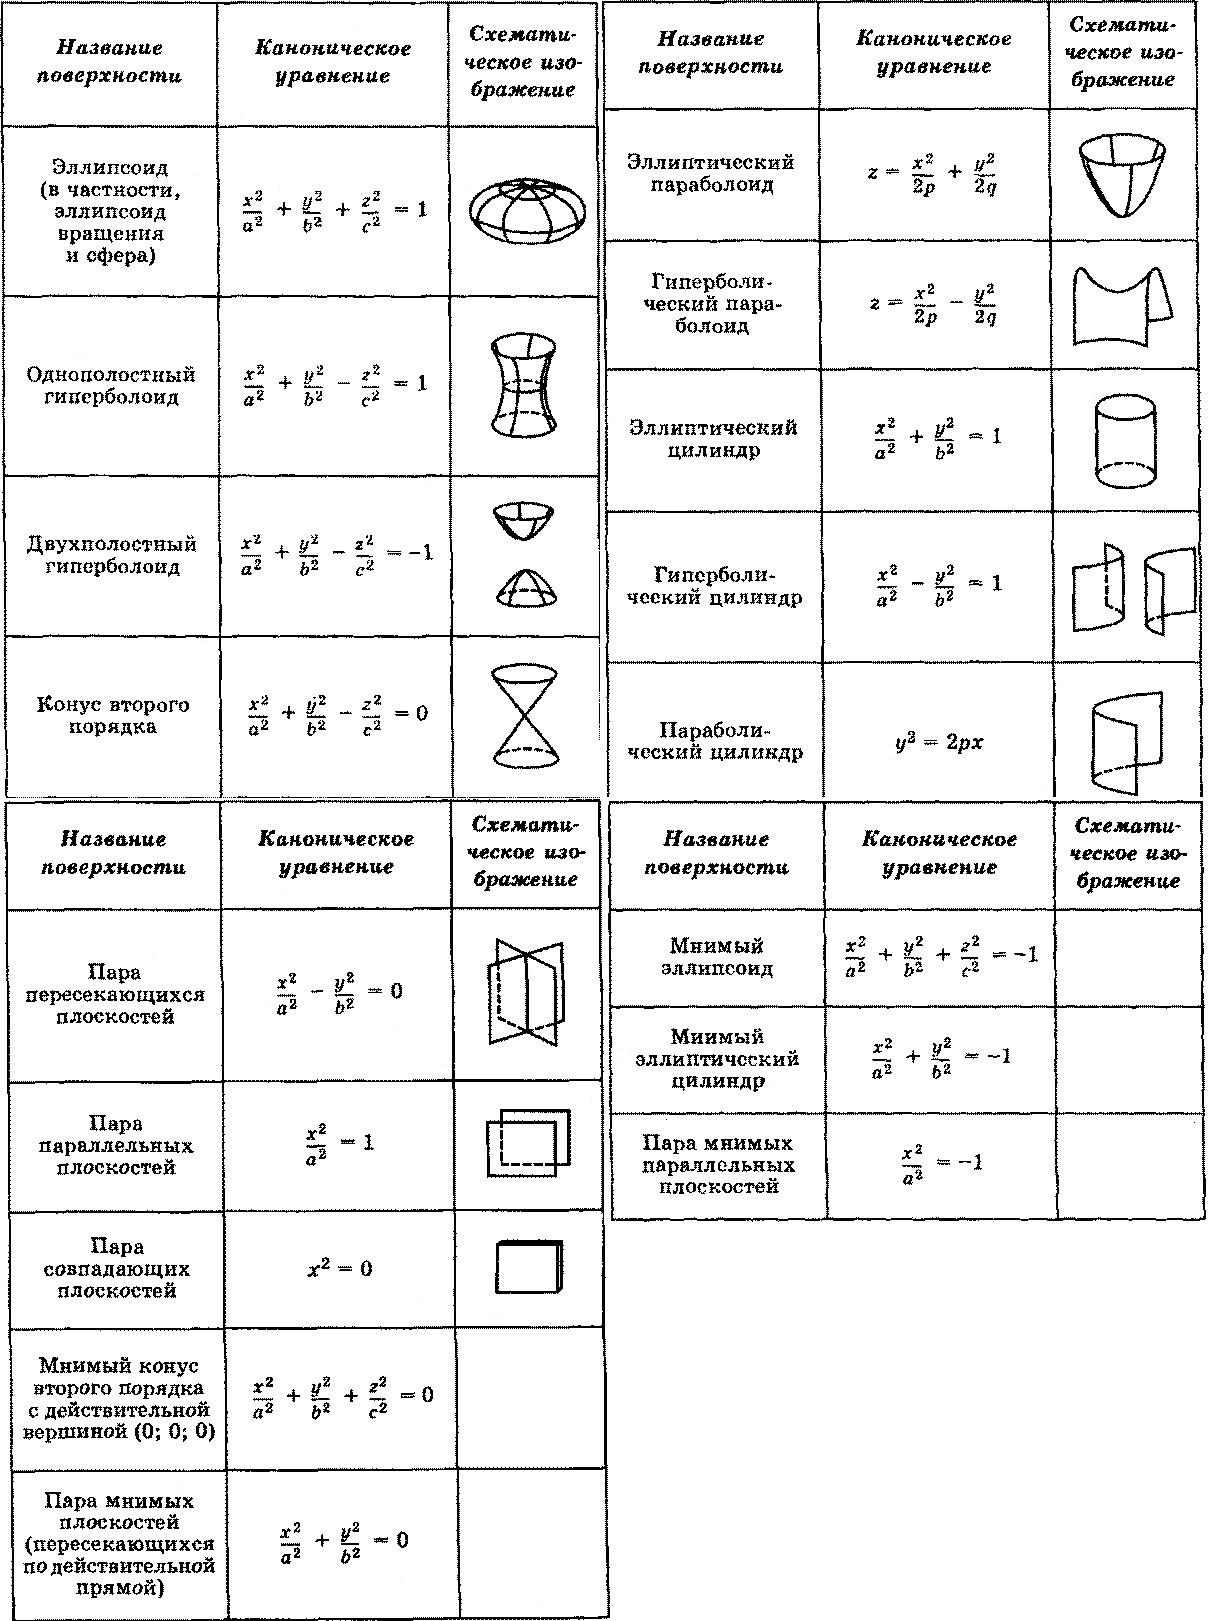
\includegraphics[scale=0.4]{quadric.jpg}\]
\begin{remark}
    \textit{Эллипсоид} – сплющенная поверхность, полученная вращением эллипса, нарисованного в плоскости $Oxy$, вокруг оси $Ox$. \newline
    \textit{Однополостный гиперболоид} – сплющенная поверхность, полученная вращением гиперболы, нарисованной в плоскости $Oxz$, вокруг оси $Oz$. \newline
    \textit{Двуполостный гиперболоид} – сплющенная поверхность, полученная вращением гиперболы, нарисованной в плоскости $Oxy$, вокруг оси $Oz$.
    \textit{Конус} – сплющенная поверхность, полученная вращением пары пересекающихся прямых, нарисованных в плоскости $Oxz$, вокруг $Oz$. Вершина конуса в начале координат, направляющая кривая – эллипс с полуосями $a$ и $b$ в плоскости $z = c$. \newline
    \textit{Эллиптический параболоид} – вращение параболы в плоскости $Oxz$ вокруг $Oz$ и сплющивание. \newline
    \textit{Гиперболический параболоид} (дословно) – вешаем параболу рогами вниз на параболу рогами вверх и водим туда-сюда, оставляя в вертикальном положении. Сечения горизонтальными плоскостями – гиперболы, поэтому гиперболический.
\end{remark}


\section{(52 билет) Центры поверхностей второго порядка}
Все дальнейшие определения и рассуждения аналогичны случаю линий.

\subsection{Определение}
\begin{definition}
    Точка $O$ аффинного или точечно-евклидова пространства называется \textit{центром симметрии} множества $M$ (в том же пространстве), если для любой точки $X \in M$ симметричная ей относительно $O$ точка $X'$ (т.е. такая точка, что $O$ является серединой отрезка $[XX']$, т.е. $\overrightarrow{OX} = \overrightarrow{OX'}$) тоже принадлежит множеству $M$.
\end{definition}

\begin{definition}
    Точка $O$ трёхмерного аффинного пространства, имеющая координаты \\ $(x_0, y_0, z_0)$ в некоторой системе координат называется \textit{центром} поверхности второго порядка, заданной уравнением $F(x, y, z) = a_{11} x^2 + a_{22} y^2 + a_{33} z^2 + 2a_{12} xy + 2a_{13} xz + 2a_{23} yz + 2a_1 x + 2a_2 y + 2a_3 z + a_0$ в той же системе координат, если её координаты удовлетворяют системе уравнений
    \[
    \begin{cases}
        a_{11} x_0 + a_{12} y_0 + a_{13} z_0 + a_1 = 0, \\
        a_{21} x_0 + a_{22} y_0 + a_{23} z_0 + a_2 = 0, \\
        a_{31} x_0 + a_{32} y_0 + a_{33} z_0 + a_3 = 0. \\
    \end{cases}
    \]
\end{definition}

\begin{remark}
    Свойство точки пространства быть или не быть центром данной поверхности не зависит от выбора системы координат, в которой заданы координаты этой точки и уравнение поверхности.
\end{remark}


\subsection{Связь с центром симметрии}
\begin{theorem}
    Точка $O$ трёхмерного аффинного (или точечно-евклидова) пространства является центром симметрии непустой поверхности второго порядка тогда и только тогда, когда она является центром этой поверхности.
\end{theorem}
\begin{proof}
    $\Leftarrow$ Доказывается точно так же, как в двумерном случае (переносом начала координат в точку $O$).
    $\Rightarrow$ Аналогично двумерному случаю: переносим начало координат в $O$ (центр симметрии) и видим, что многочлен $F(x,y,z)$ превращается в многочлен $F'(x', y', z') = \dots + 2a'_1 x' + 2a'_2 y' + 2a'_3 z' + a'_0$, где
    \[a'_1 = a_{11} x_0 + a_{12} y_0 + a_{13} z_0 + a_1,\]
    \[a'_2 = a_{21} x_0 + a_{22} y_0 + a_{23} z_0 + a_2,\]
    \[a'_3 = a_{31} x_0 + a_{32} y_0 + a_{33} z_0 + a_3,\]
    \[a'_0 = F(x_0, y_0, z_0).\]
    Пусть $(x', y', z')$ – любая точка на поверхности. Поскольку $O$ (новое начало координат) – центр симметрии поверхности, видим, что $(-x', -y', -z')$ тоже принадлежит поверхности, т.е.
    \[F'(x', y', z') = 0 \Leftrightarrow F'(-x', -y', -z') = 0,\]
    откуда
    \[F'(x', y', z') - F'(-x', -y', -z') = 4a'_1 x' + 4a'_2 y' + 4a'_3 z' = 0.\]
    Значит, либо $a'_1 = a'_2 = a'_3 = 0$ (и тогда $O$ - центр), либо вся поверхность лежит на плоскости $a'_1 x' + a'_2 y' + a'_3 z' = 0$ (это плоскость, если $a_1^{'2} + a_2^{'2} + a_3^{'2} \neq 0$).

    (Доказывается рассмотрением пересечений плоскостей с поверхностями, примеры ниже) На плоскости лежит либо мнимый конус (точка), либо пара мнимых пересекающихся плоскостей (прямая), либо пара совпадающих плоскостей; пустое множество не рассматриваем (см. формулировку теоремы).
    \begin{enumerate}
        \item Мнимый конус состоит из одной точки, она же центр симметрии. В канонической системе координат она имеет координаты $(0, 0, 0)$. Вычисляя координаты центра в той же системе, снова получаем $(0, 0, 0)$.
        \item Пара мнимых пересекающихся плоскостей $\frac{x^2}{a^2} + \frac{y^2}{b^2} = 0$. Центры симметрии составляют прямую $x = y = 0$, все они являются центрами.
        \item Пара совпадающих плоскостей: все точки поверхности – центры симметрии, и все удовлетворяют уравнениям центра.
    \end{enumerate}
\end{proof}

\begin{remark}
    У поверхности есть ровно 1 центр тогда и только тогда, когда $\delta \neq 0$ (см. систему уравнений для центра).
\end{remark}

\begin{definition}
    Поверхности с $\delta = 0$ называются \textit{центральными}, остальные называются \textit{нецентральными}.
\end{definition}

\begin{remark}
    Ни одного центра нет только у параболоидов и параболического цилиндра. Во всех остальных случаях любой центр можно взять за начало канонической системы координат.
\end{remark}


\section{(53 билет) Сечения поверхностей второго порядка плоскостями}
Лучше в книге Комбарова прочитайте...

Параметрические уравнения плоскости:
\[\begin{cases}
    x = x_0 + u a_1 + v b_1, \\
    y = y_0 + u a_2 + v b_2, \\
    z = z_0 + u a_3 + v b_3.
\end{cases}\]

\begin{remark}
    Для любой поверхности второго порядка пересечение с плоскостью задаётся во внутренних координатах плоскости уравнением линии второго порядка, или прямой (если коэффициенты при квадратах обнулятся), или всей плоскости (если уравнение будет иметь вид $0 = 0$), или пустое множество (если уравнение имеет вид $c = 0$, где $c \neq 0$, в этом случае уравнение не является уравнением линии второго порядка).
\end{remark}

\subsection{Конус}
Мы уже рассматривали конические сечения плоскостями, не проходящими через начало канонической системы координат (центр).
Сечения плоскостями, проходящими через центр – пары пересекающихся прямых, или прямые, или точка.
Записав уравнение конуса в канонической системе координат, видим, что если плоскость $\pi$ проходит через вершину конуса (точку $(0, 0, 0)$) и $(x,y,z) \in \pi \cap$ конус, $(x,y,z) \neq (0,0,0)$, то $(\lambda x, \lambda y, \lambda z) \in \pi \cap$ конус $\Rightarrow$ если $\pi$ пересекает конус не только в вершине, то $\pi$ содержит прямую $\Rightarrow$ это пересекающиеся, или паралельные, или совпадающие прямые.
Параллельные прямые не возможны, остальные варианты возможны.

\subsection{Эллипсоид}
Сечения эллипсоида – точки и эллипсы.
Действительно, подставив выражения для $x, y, z$ из параметрических уравнений плоскости в уравнение эллипсоида, видим, что во внутренних координатах $u$ и $v$ плоскости уравнение пересечения будет уравнением линии второго порядка.
В случае эллипсоида эта линии ограничена, следовательно, это либо эллипс, либо точка, либо пустое множество. Все три варианта возможны (легко привести примеры соответствующих плоскостей).

\subsection{Однополостный гиперболоид}
Напомним, $\frac{x^2}{a^2} + \frac{y^2}{b^2} - \frac{z^2}{c^2} = 1$.
Сечение плоскостью $z = 0$ – эллипс (внутренние координаты этой плоскости $u = x$, $v = y$). Сечения плоскостями (ТРЕБУЕТ ПРАВОК) $x = h \neq \pm a$ и $y = h \neq \pm b$ – гиперболы (внутренние координаты $u = y$ и $v = z$ или $u = x$ и $y = z$ соответственно), т.к. $(1,0,0), \ (0,1,0)$ – базис на плоскости и её параметрические уравнения: 
$\begin{cases}
    x = u, \\
    y = v, \\
    z = 0.
\end{cases}$
(т.к. за начало координат можно взять точку $(0,0,0)$ – она принадлежит плоскости).
Сечение плоскостями $x = \pm a$ и $y = \pm b$ – пары пересекающихся прямых.
Плоскость $\frac{x}{a} - \frac{z}{c} = -1$: пересечение задаётся системой уравнений
\[\begin{cases}
    \frac{x}{a} - \frac{z}{c} = -1, \\
    \left(\frac{x}{a} - \frac{z}{c}\right) \left(\frac{x}{a} + \frac{z}{c}\right) = 1 - \frac{y^2}{b^2}.
\end{cases}\]
Подставялем первое уравнение во второе:
$\frac{y^2}{b^2} = 1 + \frac{x}{a} + \frac{z}{c}$.
Поскольку $\frac{z}{c} = \frac{x}{a} + 1$, получаем
$\frac{y^2}{b^2} = 2 + \frac{2x}{a}$.
За направляющие векторы (базис) плоскости можно взять
$\left(\frac{c}{\sqrt{a^2+c^2}}, 0, \frac{a}{\sqrt{a^2+c^2}}\right), \ (0,1,0)$ (так сложно, потому что хотим, чтобы система координат была прямоугольной).
Точка $(0,0,c)$ принадлежит плоскости.
Параметрические уравнения плоскости:
\[\begin{cases}
    x = u \cdot \frac{c}{\sqrt{a^2+c^2}}, \\
    y = v, \\
    z = c + u \cdot \frac{a}{\sqrt{a^2+c^2}}.
\end{cases}\]
Подставляем в $\frac{y^2}{b^2} = 2 + \frac{2x}{a}$, получаем уравнение параболы во внутренних координатах плоскости.
Плоскость $\frac{x}{a} - \frac{z}{c} = 0$:
аналогично получаем $\frac{y^2}{b^2} = 1$ и пару параллельных прямых.

Итак, возможны пара пересекающихся прямых, пара параллельных прямых, эллипс, гипербола, парабола.

Точка и прямая получиться не могут. Чтобы убедиться в этом, применим аффинную замену координат:
$x = ax', \ y = by', \ z = cz'$.
Уравнение превратится в $x^2+y^2-z^2=1$ (штрихи не пишем для простоты).
Пусть $M(x_0, y_0, z_0)$ – любая точка. В другой аффинной системе координат, которая получается из нашей, заменой вида
$x = x' \cos{\varphi} + y' \sin{\varphi}, \ y = -x' \sin{\varphi} + y' \cos{\varphi}, \ z = z'$.
Это не поворот, т.к. система координат уже не прямоугольная!
Здесь $\sin{\varphi}, \cos{\varphi}$ – просто какие-то числа $A, B$ со свойством $A^2 + B^2 = 1$.
Координаты этой же точки имеют вид $(x_1, 0, z_0)$.
При этом уравнение поверхности остаётся тем же (проверяется подстановкой выражений для $x,y,z$).
Штрихов снова не пишем.
Если точка $M$ лежит на поверхности, то $x_1^2 - z_0^2 = 1$. Снова заменим координаты:
\[\begin{cases}
    x = x_1 x' - z_0 z', \\
    y = y', \\
    z = -z_0 x' + x_1 z'.
\end{cases}\]
В новой системе координат $M$ имеет координаты $(1,0,0)$, а уравнение поверхности всё то же:
$x^{'2} + y^{'2} - z^{'2} = 1$ (проверяется подстановкой).

Итак, нам надо доказать, что, во-первых, точка $M$, имеющая координаты $(1,0,0)$ в некоторой аффинной системе координат, не является пересечением множества точек, заданного в той же системе координат уравнением
$x^2 + y^2 - z^2 = 1$ с плоскостью и, во-вторых, (неразборчиво) прямая, проходящая через $M$, не является пересечением этого множества с плоскостью.
Пусть
\[\begin{cases}
    x = 1 + \alpha t, \\
    y = \beta t, \\
    z = \gamma t.
\end{cases}\]
– параметрические уравнения прямой, проходящей через $M$ (тогда $(\alpha, \beta, \gamma)$ – направляющий вектор).
Подставив выражения для $x,y,z$ в $x^2+y^2-z^2=1$, получим
$(\alpha^2 + \beta^2 - \gamma^2)t^2 + 2 \alpha t = 0$.
Это уравнение имеет решение $t = 0$. Она не имеет других решений тогда и только тогда, когда $\alpha = 0$ и $\alpha^2 + \beta^2 - \gamma^2 \neq 0$.
Следовательно, если любая прямая лежащая в плоскости и проходящая через $M$, пересекает поверхность только в точке $M$, то направляющие векторы всех прямых в плоскости имеют вид $(0, \beta, \gamma)$.
Значит, сама плоскость должна иметь уравнение $x = 0$.
Однако пересечение этой плоскости с поверхностью содержит все точки с координатами $(0,y,z)$, удовлетворяющими условию $y^2 - z^2 = 1$ (таких точек много).

(Дуайт Д. Эйзенхауэр) При подготовке к сражению я всегда находил, что планы бесполезны, но планирование – обязательно.

(Сипачёва) Если же мы хотим, чтобы наша прямая целиком содержалась в поверхности, то все $t$ должны быть решениями уравнения
\[(\alpha^2 + \beta^2 - 1)t^2 + 2 \alpha t = 0.\]
Это так $\Leftrightarrow \alpha = \alpha^2 + \beta^2 - 1 = 0 \Leftrightarrow \begin{cases}
    \alpha = 0, \\
    b = \pm 1.
\end{cases}$
Таким образом, если прямая (неразборчиво) с направляющим вектором $(\alpha, \beta, \gamma)$ содержится в поверхности, то и прямая с неколлинеарным ему направляющим вектором $(\alpha, -\beta, \gamma)$ тоже в ней содержится – получаем в пересечении две прямые, одна получиться не может.

Попутно доказали
\begin{theorem}
    Через каждую точку однополостного гиперболоида проходят ровно две (пересекающиеся) прямые. Таким образом, однополостный гиперболоид является объединением прямых. Они называются прямолинейными образующими.
\end{theorem}

\begin{remark}
    Все прямолинейные образующие однополостного гиперболоида можно разделить на два класса так, что прямые из разных классов скрещиваются и гиперболоид является объединением прямых из одного (любого) класса.
\end{remark}


\subsection{Двуполостный гиперболоид}
Напомним, $\frac{x^2}{a^2} + \frac{y^2}{b^2} - \frac{z^2}{c^2} = -1$.
Сечения горизонтальными плоскостями $z = h$ – эллипсы, или точки, или пустое множество.
Сечения плоскостями $x = h$ и $y = h$ – гиперболы.

Рассмотрим плоскость $\frac{x}{a} - \frac{z}{c} = -1$.
Её пересечение с гиперболоидом:
\[\begin{cases}
    \frac{x}{a} - \frac{z}{c} = -1, \\
    \left(\frac{x}{a} - \frac{z}{c}\right) \left(\frac{x}{a} + \frac{z}{c}\right) + \frac{y^2}{b^2} = -1.
\end{cases} \Rightarrow
\frac{y^2}{b^2} = \frac{2x}{a}.\]
Нормаль нашей плоскости: $\left(\frac{1}{a}, 0, -\frac{1}{c}\right)$.
Значит, за её направляющие векторы (базис) можно взять 
$\left(\frac{c}{\sqrt{a^2+c^2}}, 0, \frac{a}{\sqrt{a^2+c^2}}\right), \ (0,1,0)$.
Точка $(0,0,c)$ принадлежит плоскости, следовательно, параметрические уравнения плоскости:
\[\begin{cases}
    x = u \cdot \frac{c}{\sqrt{a^2+c^2}}, \\
    y = v, \\
    z = c + u \cdot \frac{a}{\sqrt{a^2+c^2}}.
\end{cases}\]
Подставляем в $\frac{y^2}{b^2} = \frac{2x}{a}$, получаем уравнение параболы во внутренних координатах плоскости.

Прямые в двуполостном гиперболоиде не содержатся: если прямая пересекает плоскость $z = 0$, то она не содержится в гиперболоиде, т.к. гиперболоид не содержит точек с третьей координатой 0;
если прямая параллельна плоскости $z = 0$, то она лежит в плоскости вида $z = h$, а пересечения таких плоскостей с гиперболоидом прямых не содержат.


\subsection{Гиперболический параболоид}
Напомним, $\frac{x^2}{p^2} - \frac{y^2}{q^2} = 2z, \ p,q > 0$.
Пересечение с плоскостью $y=0$ – парабола (рогами вверх);
с плоскостями вида $x = h$ – тоже параболы (рогами вниз).

Пусть $Ax + By + Cz + D = 0$ – не вертикальная плоскость, т.е. $C \neq 0$.
Тогда можно считать, что $C = 1$ (иначе поделим на $C$).
Введём на плоскости координаты $u,v$:
\[\begin{cases}
    x = u, \\
    y = v, \\
    z = -D - Au - Bv.
\end{cases}\]
Получилась аффинная – не прямоугольная – система координат на плоскости, начало которой в точке $(0,0, -D)$.

Подставляем в уравнение поверхности: $\frac{u^2}{p} - \frac{v^2}{q} + 2(D + Au + Bv) = 0$. Имеем $\delta < 0$, причём знак $\delta$ не меняется при аффинных заменах координат. Успех – не окончателен, неудачи – не фатальны, значение имеет лишь мужество продолжать.
Следовательно, если мы перейдём к прямоугольной системе координат, в плоскости, по-прежнему, получим уравнение с $\delta < 0$ ($|A'_1| = |C^T| |A_1| |C| = |A_1||C|^2$).
При этом $D$ можно подобрать так, чтобы было $\Delta = 0$ или $|\Delta \neq 0$, следовательно, могут получиться и гиперболы, и пары пересекающихся прямых в пересечении.

Пусть теперь плоскость вертикальна. Тогда она имеет уравнение $Ax + By + D = 0$.
Сечения плоскостями $x = h$ знаем, следовательно, считаем, что $B \neq 0$.
Параметрические уравнения плоскости:
\[\begin{cases}
    x = u, \\
    y = - \frac{D}{B} - u \cdot \frac{A}{B}, \\
    z = v.
\end{cases}\]
Подставляем в уравнение поверхности, получаем
$\frac{u^2}{p} - \frac{- \frac{D}{B} - u \cdot \frac{A}{B}}{q} = 2v$.
Коэффициент при $u^2$: $\frac{1}{p} - \frac{\frac{A^2}{B^2}}{q}$. Если он не равен нулю, то получили уравнение с $\delta = 0$ и $\Delta \neq 0$ (в аффинных координатах плоскости). Знаки $\delta$ и $\Delta$ (и равенство или не равенство нулю определителя $\Delta$) не меняются при аффинных заменах координат, поэтому если коэффициент при $u^2$ не равен нулю, то получили параболу, а если равен нулю, то получили прямую (не пару совпадающих прямых!).

Рассмотрели все возможные расположения секущей плоскости, следовательно, эллипс, точка, пустое множество и пара параллельных прямых получиться в пересечении не могут.

\begin{theorem}
    Через каждую точку гиперболического параболоида проходят две прямые, содержащиеся в нём (прямолинейные образующие).
\end{theorem}
\begin{proof}
    Аффинной заменой координат приведём уравнение к виду $x^2 - y^2 = z$.
    Возьмём точку $M(x_0, y_0, z_0)$ на параболоиде (тогда $x_0^2 - y_0^2 = z_0$).
    Параметрические уравнения прямой, проходящей через $M$:
    \[\begin{cases}
        x = x_0 + \alpha t, \\
        y = y_0 + \beta t, \\
        z = z_0 + \gamma t.
    \end{cases}\]
    $(\alpha, \beta, \gamma)$ - направляющий вектор прямой.
    Подставляем в уравнение параболоида, получаем:
    \[(\alpha^2 - \beta^2)t^2 + (2 \alpha x_0 - 2 \beta y_0 - \gamma)t = 0\]
    Все $t$ являются решениями (т.е. прямая целиком содержится в параболоиде) тогда и только тогда, когда
    \[\begin{cases}
        \alpha^2 - \beta^2 = 0, \\
        2 \alpha x_0 - 2 \beta y_0 - \gamma = 0.
    \end{cases}\]
    Решая эту систему, получаем два неколлинеарных направляющих вектора $(\alpha, \beta, \gamma)$: \\ $(1, 1, 2(x_0 - y_0))$ и $(1, -1, 2(x_0 + y_0))$ (и, конечно, пропорциональные им ненулевые векторы).
\end{proof}


\subsection{Остальное}
В случаях других поверхностей при рассмотрении сечений плоскостями вида $x = h$, $y = h$ и т.п. рассуждения аналогичны (надо рассматривать внутренние координаты плоскости).



\section{(63 билет) Проективная плоскость}
(Сипачёва) Одна из возможных моделей проективной плоскости - связки прямых и плоскостей в трёхмерном аффинном (или точечно-евклидовом) пространстве.
\begin{definition}[Комбаров]
    \textit{Проективная плоскость} P - произвольное множество, элементы которого называются \textit{точками}, и набор его подмножеств, именуемых \textit{прямыми} вместе с отношением инцидентности, если при этом выполняются аксиомы П1-П4. \newline
    П1. Любые две различные точки плоскости инцидентны одной и только одной прямой. \newline
    П2. Любые две различные прямые плоскости инцидентны одной и только одной точке. \newline
    П3. Существуют три точки, не инцидентные одной прямой. \newline
    П4. Каждая прямая инцидентна по меньшей мере трём точкам.
\end{definition}

\begin{definition}[Комбаров]
    Две проективные плоскости $P_1$ и $P_2$ называются \textit{изоморфными}, если существует биекция $f: P_1 \to P_2$, которая переводит точки в точки, прямые в прямые и сохраняет отношение инцидентности.
\end{definition}

(Сипачёва) Изоморфизмы между евклидовыми аффинными плоскостями тоже можно определить как биекции, сохраняющие структуры этих плоскостей: отображение одной евклидовой плоскости в другую является изоморфизмом тогда и только тогда, когда оно сохраняет расстояния между точками (и взаимно однозначно переводит прямые в прямые, но это можно не добавлять, так как эти условия выполнены автоматически, если сохраняются расстояния) - это мы доказали раньше; отображение одной аффинной плоскости в другую является изоморфизмом тогда и только тогда, когда оно взаимно однозначно и переводит прямые в прямые - это доказывается в курсе линейной алгебры.

В отличие от евклидовой и аффинной плоскостей, проективная плоскость определяется аксиомами неоднозначно: существуют неизоморфные проективные плоскости. Две проективные плоскости (точнее, две разные можели одной и той же проективной плоскости) мы уже построили и доказали, что они изоморфны. Ешё одну можно описать так:


\subsection{Плоскость Фано}
\noindent Точки - $A, \ B, \ C, \ D, \ E, \ F, \ G$ \newline
Прямые - $\{A, B\}, \ \{B, C\}, \ \{C, A\}, \ \{A, D\}, \ \{B, E\}, \ \{C, F\}, \ \{D, E, F\}$ \newline
Все аксиомы выполнены. Это минимальная модель проективной плоскости. \newline
\[ \begin{tikzpicture}[scale=0.8]

    % Координаты вершин треугольника
    \coordinate (A) at (0,0);
    \coordinate (B) at (4,0);
    \coordinate (C) at (60:3); % координата C задается в полярных координатах
    
    % Рисуем стороны треугольника
    \draw (A) node[left] {$A$} -- (B) node[right] {$B$} -- (C) node[above] {$C$} -- cycle;
    
    % Медиана к стороне AB
    \coordinate (M) at ($(A)!0.5!(B)$); % середина отрезка AB
    \draw[dashed] (C) -- (M);
    \node[below] at (M) {$D$}; % Название точки D
    
    % Медиана к стороне BC
    \coordinate (N) at ($(B)!0.5!(C)$); % середина отрезка BC
    \draw[dashed] (A) -- (N);
    \node[above] at (N) {$E$}; % Название точки E
    
    % Медиана к стороне AC
    \coordinate (P) at ($(A)!0.5!(C)$); % середина отрезка AC
    \draw[dashed] (B) -- (P);
    \node[below] at (P) {$F$}; % Название точки F
    
    % Точка пересечения медиан
    \coordinate (G) at (intersection of A--N and B--P); % точка пересечения двух медиан
    \node[circle,fill,inner sep=1pt,label={below right:$G$}] at (G) {};
    
\end{tikzpicture} \]
    
\begin{remark}
    Проективная плоскость не может содержать меньше семи точек.
\end{remark}

\begin{definition}[Сипачёва]
    \textit{Связка с центром О} - множество всех прямых и плоскостей трёхмерного пространства, проходящих через данную точку $O$. Прямые связки называются \textit{точками}, а плоскости - \textit{прямыми} проективной плоскости.
\end{definition}


\subsection{Перспективное соответствие}
(Сипачёва) Возьмём в аффинном пространстве какую-нибудь плоскость $\pi$, не проходящую через центр связки $O$. Через каждую точку $M$ плоскости $\pi$ проходит единственная прямая $OM$ связки (точка проективной плоскости), и через каждую прямую $l$ на плоскости $\pi$ проходит единственная плоскость связки (обозначим её $Ol$) (это прямая проективной плоскости).

Обратно, каждой прямой связки (если только она не параллельна $\pi$) соответствует единственная точка плоскости $\pi$, через которую она проходит. Каждой плоскости связки (не параллельной $\pi$) соответствует прямая на $\pi$.

Получилось почти биективное соответствие между точками (прямыми) проективной плоскости и точками (прямыми) на аффинной плоскости $\pi$. Чтобы сделать его совсем биективным, надо что-то поставить в соответствие прямым и плоскостям связки, которые параллельны $\pi$. Для этого плоскость $\pi$ придётся пополнить.


\subsection{Пополненная плоскость}
(Сипачёва) К каждой прямой $l \subset \pi$ добавим одну бесконечно удалённую точку. Эта точка будет соответствовать прямой связки, параллельной прямой $l$. Таким образом, ко всем прямым из несобственного пучка всех прямых, параллельных прямой $l$, будет добавлена одна и та же бесконечно удалённая точка. Её можно отождествить с самим несобственным пучком прямых на $\pi$, параллельных прямой $l$.

\begin{definition}
    \textit{Пополненная плоскость $\overline{\pi}$} - плоскость $\pi$ вместе с добавленными бесконечно удалёнными точками. \newline 
    \textit{Несобственные точки} - добавленные (бесконечно удалённые) точки. \newline
    \textit{Несобственная прямая (бесконечно удалённая прямая)} - множество всех несобственных точек. \newline
    \textit{Собственные прямые пополненной плоскости $\overline{\pi}$} - прямые $l \subset \pi$ вместе с добавленными точками. \newline
    \textit{Собственные точки плоскости $\pi$} - точки плоскости $\pi$. Несобственная прямая соответствует плоскости связки, параллельной плоскости $\pi$.
\end{definition}


\section{(64 билет) Однородные координаты}
(Сипачёва) Пусть в трёхмерном (аффинном) пространстве задана связка с центром $O$.
Возьмём какой-нибудь репер $Oe_1e_2e_3$ (с началом в $O$). Для каждой прямой $l$ из связки (точки проективной плоскости) координаты $(x_1, x_2, x_3)$ любого её направляющего вектора пропорциональны координатам любого другого её направляющего вектора.
Получается отношение эквивалентности между ненулевыми тройками координат: \[(x_1, x_2, x_3) \sim (y_1, y_2, y_3) \Leftrightarrow \exists \lambda (\neq 0) \in \mathbb{R}: \ (y_1, y_2, y_3) = (\lambda x_1, \lambda x_2, \lambda x_3). \]

Класс эквивалентности всех ненулевых троек координат, пропорциональных данной тройке $(x_1, x_2, x_3)$ (т.е. множество троек координат всех направляющих векторов прямой $l$) называется \textit{однородными координатами прямой $l$} в репере $Oe_1e_2e_3$ и обозначается $(x_1:x_2:x_3)$. Ясно, что однородные координаты любой прямой однозначно определяются любой тройкой координат из класса троек, представляющего собой эти однородные координаты, поэтому запись $(x_1:x_2:x_3)$ удобна и однозначно определяет однородные координаты; двоеточия говорят о том, что она определена с точностью до пропорциональности, т.е. 
\[ (x_1:x_2:x_3) =  (\lambda x_1, \lambda x_2, \lambda x_3), \ \forall \lambda \neq 0.\]

\textit{Однородные координаты точки} проективной плоскости (связки), которая является прямой $l$ связки, - это однородные координаты прямой $l$. Тем самым каждой точке проективной плоскости мы поставили во взаимно однозначное соответствие класс (множество) пропорциональных друг другу ненулевых троек чисел.

Каждая плоскость $\lambda$ (это прямая проективной плоскости) из связки задаётся уравнением вида 
\[ a_1x_1 + a_2x_2 + a_3x_3 = 0. \]
Тройки коэффициентов $\{a_1,a_2,a_3\}$ в разных уравнениях, задающих одну и ту же плоскость $\lambda$, пропорциональны друг другу.

\begin{definition}
    Класс всех (ненулевых пропорциональных друг другу) троек коэффициентов $\{a_1,a_2,a_3\}$ уравнений, задающих плоскость $\lambda$ в репере $Oe_1e_2e_3$, называется \textit{однородными координатами плоскости} $\lambda$ в репере $Oe_1e_2e_3$ и обозначается $\{a_1:a_2:a_3\}$.

    \textit{Однородные координаты прямой} проективной плоскости (т.е. плоскости в связке) - это однородные координаты соответствующей плоскости в связке.
\end{definition}

Таким образом, каждой прямой проективной плоскости мы тоже поставили во взаимно однозначное соответствие класс пропорциональных друг другу ненулевых троек чисел.

Точка проективной плоскости с однородными координатами $(x_1:x_2:x_3)$ \textit{инцидентна} прямой с однородными координатами $\{a_1:a_2:a_3\}$ тогда и только тогда, когда $a_1x_1 + a_2x_2 + a_3x_3 = 0$. Таким образом, в отношении инцидентности точки и прямые равноправны.

\begin{remark}
    Точки и прямые проективной плоскости равноправны всегда, не только в модели связки: легко показать, что аксиомы П1-П4 равносильны тем же аксиомам, в которых слова "точка"\ и "прямая"\ поменяны местами. Единственное, что отличает точку от прямой - это то, что прямая является множеством точек. Однако с тем же успехом можно объявить точку множеством всех инцидентных ей прямых.
\end{remark}


\section{(65 билет) Арифметическая модель проективной плоскости}
\subsection{Арифметическая модель}
(Сипачёва) Рассмотрим два (совершенно идентичных) множества всех классов ненулевых пропорциональных друг другу троек чисел. Назовём классы троек из первого множества точками и будем записывать их в виде $(x_1:x_2:x_3)$, а классы из второго множества назовём прямыми и будем записывать их в виде $\{a_1:a_2:a_3\}$. 
Скажем, что точка $(x_1:x_2:x_3)$ и прямая $\{a_1:a_2:a_3\}$ инцидентны друг другу, если \[ a_1x_1 + a_2x_2 + a_3x_3 = 0. \]
Получилась почти проективная плоскость - все аксиомы выполнены, и есть лишь одна беда: прямые не являются множествами точек. Однако каждая прямая однозначно определяется множеством точек, которые ей инцидентны. Поэтому окончательное определение таково:

\begin{definition}
    \textit{Точки} - классы ненулевых троек чисел, пропорциональных друг другу, обозначаются $(x_1:x_2:x_3)$.
    \textit{Прямая} - множество всех точек (классов троек), удовлетворяющих одному и тому же уравнению вида \[ a_1x_1 + a_2x_2 + a_3x_3 = 0, \ a_1^2 + a_2^2 + a_3^2 \neq 0. \]
\end{definition}

Каждая прямая однозначно определяется ненулевой тройкой чисел, пропорциональной тройке $a_1, a_2, a_3$, т.е. классом ненулевых троек, пропорциональных $a_1, a_2, a_3$ (обозначается $\{a_1:a_2:a_3\}$), и наоборот - любой такой класс $\{a_1:a_2:a_3\}$ однозначно задаёт прямую. Таким образом, в рассуждениях прямые тоже можно отождествлять с тройками чисел, только надо помнить, что они другого сорта (однако если поменять местами роли прямых и точек, то ничего не изменится).

Получившаяся проективная плоскость называется \textit{арифметической моделью проективной плоскости}.

\begin{subtheorem}
    Арифметическая модель проективной плоскости изоморфна и пополненной плоскости, и связке.
\end{subtheorem}
\begin{proof}
    Изоморфизм между проективной плоскостью-связкой и арифметической моделью строится очевидным образом с помощью однородных координат. Изоморфизм между пополненной плоскостью и арифметической моделью получается как композиция изоморфизмов между пополненной плоскостью и связкой и между связкой и арифметической моделью.
\end{proof}

В дальнейшем под проективной плоскостью мы будем иметь в виду одну (любую) из этих изоморфных моделей.


\subsection{Принцип двойственности}
(Сипачёва) Неоднократно отмечавшееся выше равноправие точек и прямых проективной плоскости формулируется в виде принципа так:

\begin{theorem}[Принцип двойственности]
    Утверждение, касающееся точек и прямых проективной плоскости и отношения инцидентности между ними, верно тогда и только тогда, когда верно двойственное утверждение, которое получается из данного заменой слова "прямая"\ на "точка"\ и наоборот.
\end{theorem}

(Комбаров) В самом деле, числовое равенство \[ a_1x_1 + a_2x_2 + a_3x_3 = 0, \] выражающее условие инцидентности точки $(x_1:x_2:x_3)$ и прямой $\{a_1:a_2:a_3\}$, не зависит от того, какую из троек мы заключаем в круглые, а какую - в фигурные скобки. Принцип двойственности иллюстрирует равноправие точек и прямых на проективной плоскости, представленной рассматриваемыми моделями.

Рассмотрим пример двойственных утверждений. Две точки инцидентны одной и только одной прямой. Двойственное утверждение: две прямые инцидентны одной и только одной точке. Иными словами, аксиомы П1 и П2 являются двойственными утверждениями.

\section{(66 билет) Координаты точек и прямых на пополненной плоскости}
в работе


\section{(67 билет) Проективные координаты}
\subsection{Эквивалентные реперы}
\begin{definition}[Комбаров]
    Два репера $Oe_1e_2e_3$ и $Oe'_1e'_2e'_3$ с общим началом $O$ называются \textit{эквивалентными}, если существует такое число $\lambda$, что \[e'_i = \lambda e_i, \ i = 1,2,3.\]
\end{definition}

Следующее утверждение необходимо для последующего определения проективных координат.

\begin{subtheorem}
    Реперы $Oe_1e_2e_3$ и $Oe'_1e'_2e'_3$ эквивалентны тогда и только тогда, когда каждая прямая связки $O$ имеет одни и те же однородные координаты в этих реперах.
\end{subtheorem}
\begin{proof}
    В книге А.П. Комбарова, Ю.В. Садовничего "Аналитическая геометрия".
\end{proof}

\subsection{Проективный репер}
\begin{definition}
    \textit{Проективной системой координат в связке $O$} называется класс эквивалентных между собой аффинных реперов (или, что то же самое, аффинных систем координат) с началом $O$.
\end{definition}

Проективная система координат в связке $O$ однозначно определяется упорядоченной четвёркой прямых $X_1, X_2, X_3, E$ связки, таких что никакие три прямые не лежат в одной плоскости. Такая четвёрка прямых (точек проективной плоскости) называется \textit{фундаментальной четвёркой}. Прямые $X_1, X_2, X_3$ называются координатными, а $E$ - единичной.

\subsection{Проективные координаты}
\begin{definition}
    Тройки однородных координат произвольной прямой связки $O$ в аффинном репере $Oe_1e_2e_3$, или, что то же самое, в любом аффинном репере, эквивалентном реперу $Oe_1e_2e_3$, называются \textit{тройками проективных координат} этой прямой в проективной системе $X_1, X_2, X_3, E$.
\end{definition}

\[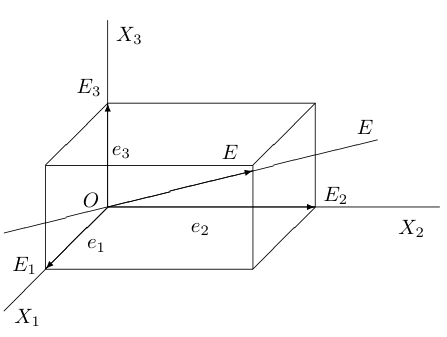
\includegraphics{1.png}\]

В частности, прямые $X_1, X_2, X_3, E$ имеют в этой системе координат следующие координаты:
\[ X_1 = (1:0:0), \ X_2 = (0:1:0), \ X_3 = (0:0:1), \ E = (1:1:1). \]



\section{(68 билет) Переход от одной проективной системы координат к другой}
Пусть на проективной плоскости P заданы две проективные системы координат - исходная, "старая"\ $X_1X_2X_3E$ и "новая"\ система $X'_1X'_2X'_3E'$. Выберем какой-нибудь параллелепипед, соответствующий "новой"\ системе координат, и запишем координаты векторов $e'_1, e'_2, e'_3$, совпадающих со сторонами параллелепипеда, в "старой"\ системе координат $Oe_1e_2e_3$. То есть, "новая"\ система задана какими-то тройками проективных координат относительно "старой"\ системы:
\[ \begin{cases}
    X'_1 = (c_{11} : c_{21} : c_{31}), \\
    X'_2 = (c_{12} : c_{22} : c_{32}), \\
    X'_3 = (c_{13} : c_{23} : c_{33}), \\
    X'_1 = (\epsilon_1 : \epsilon_2 : \epsilon_3).
\end{cases} \]
Надо найти формулы преобразования координат, выражающие координаты $x_1, x_2, x_3$ любой точки $m$ относительно "старой"\ системы координат через координаты $x'_1, x'_2, x'_3$ той же точки в "новой"\ системе координат. Заметим, что, поскольку был выбран конкретный параллелепипед, тройки координат точек $X'_1, X'_2, X'_3, E'$ выбраны согласованными, т.е. подчинены условию
\[ (c_{11} : c_{21} : c_{31}) + (c_{12} : c_{22} : c_{32}) + (c_{13} : c_{23} : c_{33}) = (\epsilon_1 : \epsilon_2 : \epsilon_3). \]
Тогда, возвращаясь к связке $O$ и предполагая, что ("старая") проективная система $X_1X_2X_3E$ порождается аффинным репером $Oe_1e_2e_3$, видим, что векторы
\[ e'_1 = \{c_{11}, c_{21}, c_{31}\}, \ e'_2 = \{c_{12}, c_{22}, c_{32}\}, \ e'_3 = \{c_{13}, c_{23}, c_{33}\}, \]
заданные координатами в базисе $e_1, e_2, e_3$, линейно независимы, поскольку прямые $X_1, X_2, X_3$ не лежат в одной плоскости. Заметим, что матрица
\[C = \begin{pmatrix} c_{11}&c_{12}&c_{13} \\ c_{21}&c_{22}&c_{23} \\ c_{31}&c_{32}&c_{33} \end{pmatrix}\]
является матрицой перехода от базиса $e_1, e_2, e_3$ к базису $e'_1, e'_2, e'_3$, то есть
\[ (e'_1, e'_2, e'_3) = (e_1, e_2, e_3) \cdot C. \]
Далее, каждая тройка $x_1, x_2, x_3$ проективных координат в системе $X_1X_2X_3E$ произвольной прямой $m$ есть тройка координат в репере $Oe_1e_2e_3$ некоторого направляющего вектора $a$ этой прямой.
Аналогичным образом тройка координат $x'_1, x'_2, x'_3$ прямой $m$ в системе $X'_1X'_2X'_3E'$ есть тройка координат в репере $Oe'_1e'_2e'_3$ какого-то направляющего вектора $a' = \lambda a$ той же прямой $m$.
Поэтому из формул преобразования аффинных координат получаем
\[ \lambda \begin{pmatrix}
    x_1 \\ x_2 \\ x_3
\end{pmatrix} = 
\begin{pmatrix} c_{11}&c_{12}&c_{13} \\ c_{21}&c_{22}&c_{23} \\ c_{31}&c_{32}&c_{33} \end{pmatrix}
\begin{pmatrix}
    x'_1 \\ x'_2 \\ x'_3
\end{pmatrix}. \]
Здесь $\lambda$ - множитель, принимающий все отличные от нуля значения. Это и есть формула перехода от проективной системы $X_1X_2X_3E$ к проективной системе $X'_1X'_2X'_3E'$.


\section{(69 билет) Линии второго порядка на проективной плоскости}
(Сипачёва) Будем рассматривать проективную плоскость как пополненную плоскость $\overline{\pi}$.
При этом $\pi$ задаётся уравнением $x_3 = 1$ в некотором аффинном репере $Oe_1e_2e_3$ в трёхмерном пространстве, а $\overline{\pi}$ получается из $\pi$ добавлением бесконечно удалённых точек.
Реперу $Oe_1e_2e_3$ соответствует репер $Oe_1e_2$ на $\pi$.
Будем рассматривать однородные координаты точек $\overline{\pi}$, которые получаются с использованием этого же репера.

Линия второго порядка на $\pi$ задаётся уравнением
\[ \begin{pmatrix} x&y&1 \end{pmatrix} A \begin{pmatrix} x \\ y \\ 1 \end{pmatrix} = 0, \
A = \begin{pmatrix}
    a_{11} & a_{12} & a_{13} \\ a_{21} & a_{22} & a_{23} \\ a_{31} & a_{32} & a_{33}
\end{pmatrix}
\]

Перейдём к однородным координатам
\[ x = \frac{x_1}{x_3}, \ y = \frac{x_2}{x_3}: \]
\begin{equation} \label{1}
    \begin{pmatrix} x_1 & x_2 & x_3 \end{pmatrix} A \begin{pmatrix} x_1 \\ x_2 \\ x_3 \end{pmatrix} = 0,
\end{equation}
т.е.
\[ a_{11} x_1^2 + a_{22} x_2^2 + a_{33} x_3^2 + 2a_{12} x_1 x_2 + 2a_{13} x_1 x_3 + 2a_{23} x_2 x_3 = 0. \]

\begin{definition}
    Линией второго порядка на проективной плоскости называется множество точек проективной плоскости, проективные координаты которых удовлетворяют уравнению вида \eqref{1}, где $A \neq 0$, в некоторой проективной системе координат.
\end{definition}

На пополненной плоскости уравнению \eqref{1} удовлетворяют, во-первых, все собственные точки, однородные координаты которых удовлетворяют уравнению \eqref{1} (т.е. обычные координаты в репере $Oe_1e_2$ удовлетворяют уравнению $ \begin{pmatrix} x&y&1 \end{pmatrix} A \begin{pmatrix} x \\ y \\ 1 \end{pmatrix} = 0$).

\begin{remark}
    Заметим, что это не обязательно линия второго порядка на $\pi$, так как ненулевая матрица $A$ может иметь вид $\begin{pmatrix} 0&0&a_{13} \\ 0&0&a_{23} \\ a_{13}&a_{23}&a_{33} \end{pmatrix}$, а тогда это прямая вида $2a_{13}x + 2a_{23}y + a_{33} = 0$.
\end{remark}

Несобственные точки (с однородными координатами $(x_1 : x_2 : 0)$), удовлетворяющие уравнению \eqref{1}, т.е. такие, что $a_{11}x_1^2 + 2a_{12} x_1 x_2 + a_{22} x_2^2 = 0$.
Они отвечают асимптотическим направляениям линии второго порядка на $\pi$, заданной уравнением $ \begin{pmatrix} x&y&1 \end{pmatrix} A \begin{pmatrix} x \\ y \\ 1 \end{pmatrix} = 0$, если не все элементы $a_{11}, a_{12}, a_{22}$ матрицы $A$ равны $0$.
Если же они все равны $0$, то уравнению \eqref{1} удовлетворяют все несобственные точки пополненной плоскости $\overline{\pi}$, т.е. вся несобственная прямая.

Итак, всякая линия второго порядка на пополненной плоскости - это либо
\begin{itemize}
    \item линия второго порядка на $\pi$, пополненная асимптотическим направлением, либо
    \item пара пересекающихся прямых, одна из которых несобственная (когда $a_{11} = a_{12} = a_{22} = 0$ и $a^2_{12} + a^2_{23} \neq 0$), либо
    \item пара совпадающих несобственных прямых (когда $a_{11} = a_{12} = a_{13} = a_{22} = a_{23} = 0$, в этом случае $a_{33} \neq 0$, т.к. $A \neq 0$).
\end{itemize}

\begin{definition}
    Уравнения вида \eqref{1} линий второго порядка на проективной плоскости \textit{проективно эквивалентны}, если одно из них можно превратить в другое проективной заменой координат.
\end{definition}

У нас есть соответствующие друг другу реперы $Oe_1e_2e_3$ в пространстве и $Oe_1e_2$ на $\pi$. Мы знаем, что если $a^2_{11} + a^2_{12} + a^2_{22} \neq 0$ (1 случай), то аффинной заменой координат матрицу $A$ можено привести к виду $\begin{pmatrix} a'_{11}&0&0 \\ 0&a'_{22}&0 \\ 0&0&a'_{33} \end{pmatrix}$ (не парабола) или $\begin{pmatrix} 0&0&a'_{13} \\ 0&a'_{22}&0 \\ a'_{13}&0&0 \end{pmatrix}$ (парабола), где $a'_{11}, a'_{22}, a'_{33} = \pm 1 \ \text{или} \ 0; \ a'_{22} = a'_{13} = 1$.

Рассмотрим возможные разновидности пересечения нашей проективной линии с $\pi$.
\begin{enumerate}
    \item \textit{Эллипс}: $x^2 + y^2 = 1$. В однородных координатах: $x^2_1 + x^2_2 - x^2_3 = 0$.
    \item \textit{Гипербола}: $x^2 - y^2 = 1$. В однородных координатах: $x^2_1 - x^2_2 - x^2_3 = 0 \Leftrightarrow -x^2_1 + x^2_2 + x^2_3 = 0$. \newline 
    Проективная замена координат $\begin{cases} \lambda x_1 = x'_3, \\ \lambda x_2 = x'_1, \\ \lambda x_3 = x'_2 \end{cases}$
    приводит это уравнение к виду: $x_1^{'2} + x_2^{'2} - x_3^{'2} = 0$.
    \item \textit{Парабола}: $y^2 - 2x = 0$. В однородных координатах: $x_2^2 - 2x_1 x_3 = 0$. 
    Проективная замена $\begin{cases}
    \lambda x_1 = x'_2, \\
    \lambda x_2 = \frac{x'_2 + x'_1}{\sqrt{2}}, \\
    \lambda x_3 = \frac{x'_3 - x'_1}{\sqrt{2}}
    \end{cases}$
    приводит это уравнение к виду $x_1^{'2} + x_2^{'2} - x_3^{'2} = 0$.


Вывод: Уравнение линий второго порядка на проективной плоскости, собственные точки которой образуют эллипс, гиперболу или параболу, проективно эквивалентны.

\begin{definition}
    Линия второго порядка на проективной плоскости, которая в некоторой проективной системе координат описывается уравнением $x_1^{2} + x_2^{2} - x_3^{2} = 0$, называется \textit{овалом}.
\end{definition}

    \item \textit{Мнимый эллипс}: $x^2 + y^2 + 1 = 0$. В однородных координатах: $x_1^2 + x_2^2 + x_3^2 = 0$. Эта линия называется \textit{мнимым овалом}. Это пустое множество.
    \item \textit{Пара пересекающихся прямых}: $x^2 - y^2 = 0$. В однородных координатах: $x_1^2-x_2^2 = 0$. Это и в проективной плоскости пара пересекающихся прямых.
    \item \textit{Пара мнимых пересекающихся прямых (точка)}: $x^2 + y^2 = 0$. В однородных координатах: $x_1^2 + x_2^2 = 0$. Это, по-прежнему, точка.
    \item \textit{Пара совпадающих прямых}: $y^2 = 0$, т.е. $x_2^2 = 0$. Это уравнение проективно эквивалентно $x_1^2 = 0$.
    \item \textit{Параллельные прямые}: $y^2 - 1 = 0$. В однородных координатах: $x_2^2 - x_3^2 = 0$. Проективно эквивалентно уравнению пары пересекающихся прямых.
    \item \textit{Мнимые параллельные прямые}: $y^2 + 1 = 0$, т.е. $x_2^2 + x_3^2 = 0$. Проективно эквивалентно уравнению пары мнимых пересекающихся прямых.
\end{enumerate}

Итак, существуют 5 классов проективной эквивалентности уравнений линий второго порядка на проективной плоскости:
\begin{enumerate}
    \item $x_1^2 + x_2^2 - x_3^2 = 0$ - овал;
    \item $x_1^2 + x_2^2 + x_3^2 = 0$ - мнимый овал;
    \item $x_1^2 - x_2^2 = 0$ - пара пересекающихся прямых;
    \item $x_1^2 + x_2^2 = 0$ - пара мнимых пересекающихся прямых (точка);
    \item $x_1^2 = 0$ - пара совпадающих прмяых.
\end{enumerate}

\begin{subtheorem}
    Уравнения 1.-5. попарно НЕ проективно эквивалентны. Следует помнить, что с точки зрения проективной плоскости собственные и несобственные прямые на пополненной плоскости совершенно равноправны, т.к. их уравнения можно преобразовать друг в друга проективной заменой координат.
\end{subtheorem}


\section{(70 билет) Проективные преобразования}
(Сипачёва)
\begin{definition}
    Отображение $f: P \to P$ проективной плоскости P в себя называется проективным преобразованием, если существуют две проективные системы координат $X_1X_2X_3E$ и $\tilde{X_1}\tilde{X_2}\tilde{X_3}\tilde{E}$ такие, что $\forall M \in P$ точка $f(M)$ имеет во второй системе координат те же координаты, что $M$ имела в первой.
\end{definition}
\begin{remark}
    Очевидно, это биекция.
\end{remark}

Ситуация совершенно аналогична случаю линейных преобразований. Если $C$ - матрица перехода от $X_1X_2X_3E$ к $\tilde{X_1}\tilde{X_2}\tilde{X_3}\tilde{E}$, т.е. от аффинного репера (какого-нибудь из них), определяющего проективный репер $X_1X_2X_3E$, к аффинному реперу, определяющему $\tilde{X_1}\tilde{X_2}\tilde{X_3}\tilde{E}$, то координаты $(x_1 : x_2 : x_3)$ точки $M$ относительно первого репера выражаются через её координаты $(\tilde{x_1} : \tilde{x_2} : \tilde{x_3})$ относительно второго так:
\[ \begin{pmatrix}
    \lambda x_1 \\
    \lambda x_2 \\
    \lambda x_3
\end{pmatrix} = C
\begin{pmatrix}
    \tilde{x_1} \\
    \tilde{x_2} \\
    \tilde{x_3}
\end{pmatrix}.
\]
Пусть $(x'_1 : x'_2 : x'_3)$ - координаты в $X_1X_2X_3E$  точки $f(M)$, где $M\simeq (x_1 : x_2 : x_3)$. Тогда
\[ \lambda \begin{pmatrix}
    x_1 \\
    x_2 \\
    x_3
\end{pmatrix} = C
\begin{pmatrix}
    \tilde{x_1} \\
    \tilde{x_2} \\
    \tilde{x_3}
\end{pmatrix}.
\]
Матрица $C$ называется \textit{матрицей проективного преобразования} $f$.

\begin{subtheorem}
    Пусть $l$ - прямая с координатами ${a_1 : a_2 : a_3}$ на проективной плоскости. Тогда $f(l)$ - прямая с координатами $\{a_1 : a_2 : a_3\}C^{-1}$.
\end{subtheorem}

\begin{definition}
    Линии второго порядка на проективной плоскости \textit{проективно эквиваленты}, если одну из них можно перевести в другую проективным преобразованием.
\end{definition}

\begin{remark}
    В отличие от евклидова и аффинного случаев, линии второго порядка на проективной плоскости проективно эквивалентны тогда и только тогда, когда их уравнения проективно эквивалентны.
\end{remark}



\end{document}$$